

\subsection{$^{83m}$Kr as an electric field probe} \label{section:S1aS1b1}


$^{83m}$Kr is ideally suited as a probe of the TPC electric field. As a short lived noble gas, 
it can be injected frequently into the detector without harm, and it mixes uniformly 
into the detector volume within minutes. Efficiency effects cancel in the S1a/S1b ratio, 
because the two decays occur at the same location in the detector. 
Both decays are electron events, so the only variable in
the S1a/S1b ratio, besides statistical fluctuations, is the magnitude of the electric field at the decay location.

In this section we report the relationship between S1a/S1b and the absolute electric field as 
calculated by the COMSOL field model described in Ref.~\cite{lucie}. Knowledge of the absolute electric field and its 
relationship to S1a/S1b is useful for comparing LUX data to predictions from the NEST framework, 
however it is not critical for applying efficiency corrections to the LUX WIMP search. 
As described in Sec.~\ref{sec:corrections}, we directly characterize those corrections as 
functions of S1a/S1b alone.

We select $^{83m}$Kr events with exactly one S2 between 2000 to 60000~phd, and one or more S1 candidates 
greater than 10~phd occurring before the S2. We fit a double exponential to the S1 candidates and 
extract their pulse area and the time between decays. To ensure a good measurement of the 
S1a and S1b pulse areas, we require the time difference to be greater than 130~ns. As shown
in Fig.~\ref{fig:sumpod}, the S1 waveforms from a typical $^{83m}$Kr event show distinct
(a) and (b) decays because the scintillation time constant and detector response time is
tens of nanoseconds, substantially shorter than the 154~nanosecond half life of the $^{83m}$Kr
intermediate state. The S2 waveforms, however, represent the sum of the charge from both decays, because
the anode collection time is several microseconds.



%Once we have measured the strength of the field effect from the $^{83m}$Kr S2$_E$ data at one point in time, we need to develop a method to track the field effect at all points in time.  To accomplish this, we use the uncorrected S1 pulse area from the 32.1 keV and 9.4 keV decays within $^{83m}$Kr events, referred to as S1a and S1b respectively.  As discussed in section \ref{section:Intro}, as the electric field increases the probability of recombination decreases, leading to a smaller S1 signal.  The S1a decay is more sensitive to this effect due to its higher energy, leading to a stronger field effect in the S1a data than in the S1b data.   Therefore, an inverse relationship exists between the strength of the field and the S1a/S1b ratio.  

%comment: the S2 pulse are selection is made on S2bottom.




\begin{figure}
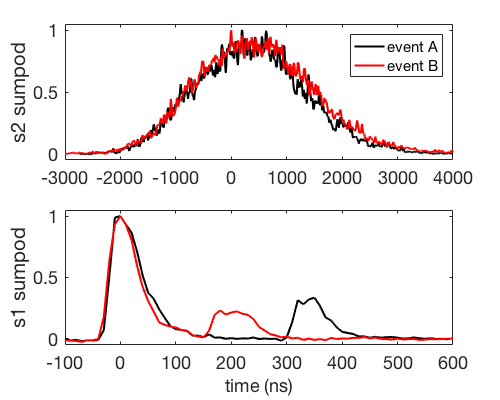
\includegraphics[scale=0.4]{figures/Fig2.png}
\captionof{figure}{S2 (upper) and S1 (lower) PMT waveforms from a typical $^{83m}$Kr decay, normalized to one. Two events with differing decay times are shown. Note the distinct time scales on the S2 and S1 plot axes. The 32.1~keV and 9.4~keV decays are distinct in S1, but are summed together in S2 due to the $\sim$microsecond collection time of the S2 anode region. Although the S2 signals are required to follow the S1 signals in time, for clarity the S2 signals are shown here centered on $t=0$.}
 \label{fig:Sumpod}
\end{figure}

We construct an S1a/S1b map for the September 2015 calibration data by dividing the detector into three dimensional voxels 
of XXX x YYY x ZZZ dimension. We fit Gaussians to the S1a and S1b histograms in each voxel and take the ratio of the fitted means.  
Figure~\ref{fig:s1as1bmap} shows the resulting map, which is observed to follow closely the electric field pattern from the COMSOL model for the same date.
 A scatter plot of the electric field vs S1a/S1b in each detector voxel for the September 2015 data is shown in Figure~\ref{fig:s1as1bvsfield}.
As expected, an inverse relationship is observed, since higher electric fields reduce the light yield of the 32.1~keV (a) decay 
much more than that of the 9.4~keV (b) decay. The same functional form is 
replicated in other $^{83m}$Kr datasets collected throughout the physics run under 
varying electric field conditions. 
We fit a function to the September 2015 data as shown in the Figure and find XXXXX.





%\begin{figure} [!h]
%\centering
%\subfloat{{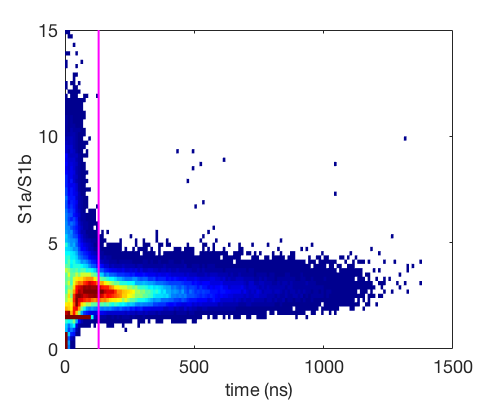
\includegraphics[width=7cm]{figures/Fig3a.png} }}
%\qquad
%\subfloat{{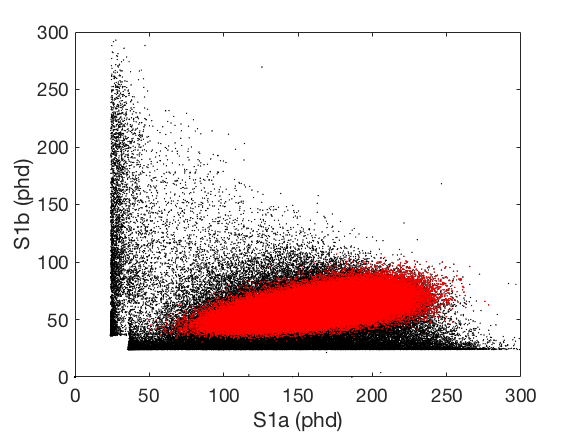
\includegraphics[width=7cm]{figures/Fig3b.png} }}
%\caption{ (Top) The output of the S1a/S1b fitting module as a function of time separation between the two decays.  The red line indicate the minimum separation between the S1a and S1b events required by our cut in this analysis. (Bottom) A scatter plot of all S1a and S1b pulse areas measured by the fitting module (black) compared to the S1a and S1b pulse areas that are left after our selection cut. (red)}
%\label{fig:S1aS1btiming}
%\end{figure}






\section{Signal Corrections in a Nonuniform Drift Field}\label{section:GenStrat}

In LUX's WS2014–16 data, pulse area corrections must account for field effects as a function of time, space, energy, and recoil type.  Since the recoil type of an event in WIMP search data is unknown, and the energy of an event in WIMP search data is unknown prior to pulse area corrections being applied, it is not possible to remove the spatial and time dependence induced by the field effects in our data.  Instead, we seek to separate the field effects from the detector inefficiency effects at the known energy and recoil type of $^{83m}$Kr, so that we can extract detector efficiency corrections that are applicable to all events from said data.  This separation must be performed at all points in time due to the time dependence of the electric field.  To accomplish this we relate the strength of the field effects in the S1 and S2 pulse areas of $^{83m}$Kr calibration data to the ratio of the two S1 pulses (referred to as S1a and S1b) generated during the $^{83m}$Kr decay.  This ratio is strongly correlated with the strength of the electric field, since the two $^{83m}$Kr decays have different energies (32.1 keV for S1a and 9.4 keV for S1b) and are therefore effected by the field effects by different amounts.  Note that corrections which perfectly separate field effects from detector inefficiency effects in this manner, and only correct for the latter, will have a spatial and time dependence left in the S1 and S2 signals but not in the energy spectra or gain factors for any data, regardless of energy or recoil type.

The general strategy for measuring and separating the electric field effects in $^{83m}$Kr calibrations is as follows.  First, we measure the electric field in the detector at a particular point in time, using the methods described in reference \ref{LuciesPaper}.  We would like to use this field map in conjunction with NEST to remove the field effects in the $^{83m}$Kr data directly before measuring detector inefficiency effects.  Unfortunately, due to the complicated nature of the $^{83m}$Kr decay NEST does not accurately simulate $^{83m}$Kr data.  Instead we turn to CH$_3$T data, which NEST has been tuned to simulate extremely well.  

After using NEST to determine and remove the strength of the field effects in CH$_3$T data we measure the residual pulse area variation in the S2 signal and produce corrections for these effects, which, since the field effects have been removed, are due to detector inefficiencies alone.  These detector inefficiency corrections are equivalent to the Run03 corrections which were obtained directly from $^{83m}$Kr data in~\cite{Run03Reanalysis}.  Next, we apply the detector inefficiency corrections to contemporaneous $^{83m}$Kr data.  At this point, any residual pulse are variation in the $^{83m}$Kr S2 signal is due to field effects alone.  We measure the strength of the field effects by fitting Gaussian distributions to the inefficiency corrected $^{83m}$Kr S2 signal over a three dimensional map, choosing the ratio S2(XYZ)/S2(Center) as the figure of merit for the strength of the field effect.  At the same time we measure a three dimensional map of the $^{83m}$Kr S1a/S1b ratio.  Relating these two maps allows us to determine the strength of the field effect on $^{83m}$Kr S2 data taken at any time or location by simply measuring the $^{83m}$Kr S1a/S1b ratio. 


The same process can not be repeated for the S1 signal, since the maximum of the CH$_3$T S1 spectrum falls below the detector threshold, and there are no discernible features to extract detector inefficiency corrections from.  Instead, three approaches have been taken to measure the relationship of the field effect in inefficiency corrected $^{83m}$Kr S1 data, as measured by S1(XYZ)/S1(Center), to the $^{83m}$Kr S1a/S1b ratio.  The first approach, in section \ref{section:S1relation}, converts the S2 field effect relationship to an S1 field effect relationship using the physics behind recombination.  In section \ref{MatthewsIdea} we use the expected light yield of the $^{83m}$Kr 31.2 keV decay as a function of electric field to measure detector inefficiency effects and separate them from the field effect we want to measure.  The final approach, in section \ref{section:S1relation2}, takes advantage of the fact that the energy spectrum of any event should remain insensitive to any recombination variation that arises from a non-uniform electric field.  In this method, we float the $^{83m}$Kr S1(XYZ)/S1(Center) to S1a/S1b relationship in a $\chi^2$ fit.  Within the fit we remove the field effect in both the S1 and S2 $^{83m}$Kr data (using the floated relationship for the S1 field effect), produce inefficiency-only corrections from the data, and then evaluate the corrected $^{83m}$Kr and CH$_3$T energy spectra.  The  S1(XYZ)/S1(Center) to S1a/S1b relationship which produces the minimum $\chi^2$ between the observed and expected energy spectra is chosen as the correct relationship.

Once the field induced S2(XYZ)/S2(Center) to S1a/S1b relationship and the field induced S1(XYZ)/S1(Center) to S1a/S1b relationship have been determined they can be used in $^{83m}$Kr data sets from any time to remove the field effects in the $^{83m}$Kr data via mapping the S1a/S1b ratio.  Once the field effects are removed the residual S1 and S2 variation in the $^{83m}$Kr can be used to calculate pulse area corrections based on detector inefficiencies alone. The following sections detail each step of the process outlined above.

\subsection{Measuring Detector Inefficiency Corrections with CH$_3$T}

The first step in measuring the strength of field effects in $^{83m}$Kr calibration data is to extract detector inefficiency corrections from contemporaneous CH$_3$T data.  We use data from the September 2015 CH$_3$T calibration due to its high statistics ($\sim$300,000 events). 

Before measuring detector inefficiency corrections from CH$_3$T, we must remove the field effects from the data.   The electric field at the location of each CH$_3$T event is estimated by interpolating the electric field map from~\cite{LuciesPaper}.  A cubic interpolation is used for events which fall within the bounds of the field map, and a nearest neighbor extrapolation is used for events which fall outside of the bounds.   

Once the field strength at the location of a particular event is determined it is converted to a measurement of the recombination for each event using the following equations from the NEST framework:
\begin{align}
N_q &= \frac{E}{0.0137} \label{NqEq} \\
N_{ion} &= \frac{N_q}{1+\alpha} \label{NionEq} \\
R &= 1-\mbox{ln} \left( \frac{1+(\frac{TI*N_{ion}}{4})}{(\frac{TI*N_{ion}}{4})} \right)
\end{align}
where $E$ is the energy of the event, $N_q$ is the number of quanta, $N_{ion}$ is the number of ions, $\alpha$ is the exciton to ion ratio (assumed to be 0.11), $TI$ is the Thomas-Imel Box parameter, and $R$ is the recombination probability.  Since we do not know the energy of the event ahead of time (since we do not have working corrections at this point) we assume the most probably energy from the CH$_3$T energy spectrum, which is 2.5 keV.  We are mainly interested in fitting the maximum of the spectrum when measuring detector inefficiency corrections, so the fact that this recombination estimate for higher energy CH$_3$T events may be wrong is not concerning.  

A normalization factor $N_{photon-center}/N_{photon}$ for the S1 signal is determined by calculating the number of photons produced in events at the center of the detector, and the number of photons produced in a particular event by using
\begin{equation}
N_{photon} = N_q\frac{\alpha}{1+\alpha} + N_{ion}R
\end{equation}
Since we assumed a value of 2.5 keV for all events, the normalization constant only has a dependence on the estimated field strength at each location in the detector.  

Similarly, we determine a normalization factor $N_{elec-center}/N_{elec}$ for the S2 signal by calculating the number of electrons at the center of the detector and the number of electrons for a particular event by using the equation
\begin{equation}
N_{elec}=N_q-N_{photon}
\end{equation}
which again is only dependent on the estimated field strength at each location in the detector.  

We multiply the raw S1 and S2 signals by these normalization factors to remove the field effects from the CH$_3$T data.  For clarity, we define the field effect removed S1 and S2 signals as S1$_F$ and S2$_F$, respectively, where the subscript $F$ stands for "field corrected".   
\begin{align}
S2_F &=S2 \left( \frac{N_{elec-center}}{N_{elec}} \right) \\
S1_F &=S1 \left( \frac{N_{photon-center}}{N_{photon}} \right)
\end{align}
Likewise, we define the detector inefficiency corrected S1 and S2 signals (with field effects still present) as S1$_E$ and S2$_E$, where the subscript $E$ stands for "efficiency corrected."

After removing the field effects from the CH$_3$T data we are ready to measure the residual spatial pulse area variation due to detector inefficiencies alone.  We first measure the Z dependence of the S2$_F$ pulse area by slicing the detector into drift time bins of 10 $\mu$second width.  A Landau distribution is fit to the S2$_F$ spectrum of each bin to determine the location of the spectra maximums.  A cubic interpolation is used to determine the S2$_F$ Z dependence between each drift time bin, and a linear extrapolation based on the first and last 20\% of data points is used to determine the S2$_F$ Z dependence above and below the span of the drift time bins.  A detector inefficiency correction for the Z direction, defined as $\epsilon_{(S2,Z)}$, is measured by taking the ratio of the S2$_F$ pulse area at a height of 4 $\mu$seconds (just below the liquid surface) to the S2$_F$ pulse area as described in the equation
\begin{equation}
\epsilon_{(S2,Z)}= \frac{S2_F(z=4)}{S2_F(z)}.
\end{equation} 


The XY dependence of the field removed S2$_F$ signal, defined as $\epsilon_{(S2,XY)}$, is found by dividing the Z inefficiency corrected (S2$_F \times \epsilon_{(S2,Z})$) data into two dimensional XY bins with lengths of 3 cm on each side, and then fitting Landau distributions to the data of each bin.  The maximum of the Landau distribution from each bin is used to construct an S2$_F$ XY dependence map, with a spline interpolation and extrapolation being used to determine the XY dependence between and outside of the bins.  A detector inefficiency correction for the XY direction is defined by taking the ratio of the z inefficiency corrected S2$_F$ pulse area at the center of the detector to the z inefficiency corrected S2$_F$ pulse area as a function of XY in cm, as shown below
\begin{equation}
\epsilon_{(S2,XY)} = \frac{\epsilon_{(S2,Z)} \times S2_F(x_c,y_c,z)} { \epsilon_{(S2,Z)} \times S2_F(xyz)}.
\end{equation} 
where $x_c$ and $y_c$ are the x and y center of the detector in uncorrected coordinates determined by taking the average position of the CH$_3$T events in each direction.



Multiplying the raw S2 signal by both the Z and the XY correction factors results in an inefficiency corrected S2$_E$ signal (with field effects still present), 
\begin{equation}\label{E_eq}
S2_E =S2 \times \epsilon_{(S2,Z)} \times \epsilon_{(S2,XY)} 
\end{equation}

We are unable to directly measure the detector inefficiency corrections for the S1 signal from CH$_3$T data, since the maximum of the S1 spectrum falls below the detector threshold and there are no discernible features to fit to. Instead, we will continue working with the S2 signal of our data and return to the issue of S1 corrections in sections \ref{section:S1relation,MatthewsIdea,section:S1relation2}.


 
\subsection{Measuring Field Effects in $^{83m}$Kr S2 Data} \label{section:FieldEffects}

After measuring the S2 detector inefficiency corrections in CH$_3$T data we have all the tools we need to measure the field effects in the S2 pulse area of $^{83m}$Kr data.  We begin by applying the S2 detector inefficiency corrections to contemporaneous,  uncorrected $^{83m}$Kr data by using equation \ref{E_eq}.  The removal of the detector inefficiency effects from the raw S2 data leave us with an S2$_E$ signal which has spatial pulse area variation from field effects alone.

The process for measuring the field effects in the inefficiency corrected $^{83m}$Kr S2$_E$ data is similar to the process of measuring the detector inefficiency effects in the field effect corrected CH$_3$T S2$_F$ data.  First, we measure the field induced Z dependence of the $^{83m}$Kr S2$_E$ pulse area by slicing the detector into drift time bins of 10 $\mu$second width.  A Gaussian distribution is fit to the S2$_E$ spectrum of each bin to determine the mean S2$_E$ pulse area versus Z.   A cubic interpolation is used to determine the S2$_E$ Z dependence between each drift time bin, and a linear extrapolation based on the first and last 20\% of data points is used to determine the S2$_E$ Z dependence above and below the span of the drift time bins.  

We define the strength of the field effect in the z direction as the ratio of the S2$_E$ pulse area as a function of Z to the S2$_E$ pulse area at the center of the detector $z_c$, S2$_E$(z)/S2$_E$(center).  An S2 field effect correction for the Z direction, defined as $\eta_{(S2,Z)}$, is measured by taking the inverse of the strength of the field effect, 
\begin{equation}
\eta_{(S2,Z)} = \frac{S2_E(z=z_c)}{S2_E(z)}.
\end{equation} 

We also take a separate, three dimensional approach to mapping the field effect in the $^{83m}$Kr S2$_E$ data. In this approach the detector is divided into three dimensional voxels, with X and Y width of 3.5 cm and Z width of 30 $\mu$seconds.  As in the one dimensional case, a three dimensional map of the field induced S2$_E$ pulse area variation is produced by fitting a Gaussian distribution to the $^{83m}$Kr S2$_E$ data in each voxel.  A spline interpolation is used to determine the S2$_E$(xyz)/S2$_E$(center) ratio between the three dimensional voxels, and the S2$_E$(xyz)/S2$_E$(center) Z dependence map is used to extrapolate outside of the range of the voxels.  As shown in Figure~\ref{fig:S1aS1bField_S2}, the results are consistent between both measurements.
\subsection{Relating the S1a/S1b Ratio to S2 Field Effects} \label{section:S1aS1b2}

To relate the S1a/S1b ratio to the S2 field effects measured in section \ref{section:FieldEffects} we begin by measuring the spatial dependence of the S1a/S1b ratio.  We first divide the detector into drift time bins of 3 $\mu$second width.   A Gaussian distribution is fit to the S1a and S1b spectrum of each bin to determine the mean pulse areas versus Z.   A second order polynomial is fit to the ratio of the Gaussian means versus Z and is used to determine the S1a/S1b ratio at any drift time in the detector.  

As we did when measuring the strength of the field effect, we also take a separate, three dimensional approach to mapping the $^{83m}$Kr S1a/S1b ratio throughout the detector. In this approach the detector is divided into three dimensional voxels, with X and Y width of 3.5 cm and Z width of 30 $\mu$seconds.  A three dimensional map of S1a/S1b is produced by fitting a Gaussian distribution to the S1a and S1b pulse area spectrum in each voxel.  A spline interpolation and extrapolation is used to determine the S1a/S1b ratio between and outside of the three dimensional voxels.

We relate the Z dependence and three dimensional dependence maps of the S1a/S1b ratio to the Z dependence and three dimensional dependence maps of the S2 field effect measured in section \ref{section:FieldEffects}.  A second order polynomial is fit to the spatial dependence of the $^{83m}$Kr S2$_E$ (induced by the field effect) to S1a/S1b relationship, with best fit parameters of $a=-0.499 \pm 0.117$,$b=1.48 \pm 0.615$, and $c=0.667 \pm 0.946$ for the second order, first order, and zeroth order terms, respectively. This polynomial is used to determine the strength of the field effect in $^{83m}$Kr S2 data at all points in time.  We find that the Z dependence and three dimensional maps agree closely within the range of measured S1a/S1b ratios, but begin to diverge in the extrapolated regions (Figure \ref{fig:S1aS1bField_S2}). 

\begin{center}
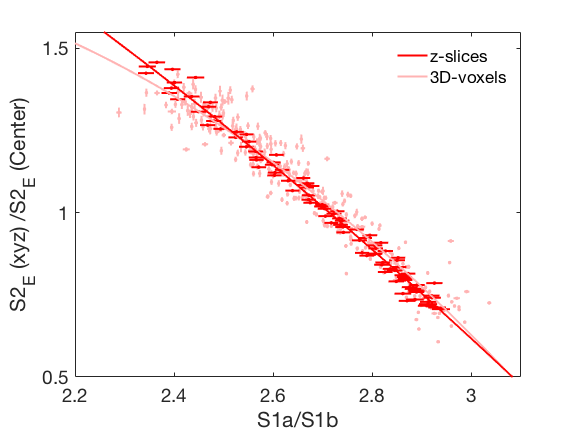
\includegraphics[scale=0.4]{figures/Fig4.png}
\captionof{figure}{The Z (dark red) and three dimensional (light red) relationship of the $^{83m}$Kr S1a/S1b ratio to the $^{83m}$Kr S2$_E$ field effect.}
 \label{fig:S1aS1bField_S2}
\end{center}

\subsection{Measuring the S1a/S1b Ratio to S1 Field Effect Relationship with Recombination Physics} \label{section:S1relation}

We have successfully measured the strength of the field effect in $^{83m}$Kr S2 data at one point in time, and have related it to the $^{83m}$Kr S1a/S1b ratio such that we can determine the strength of the field effect at any point in time.  We are now left with the challenge of measuring the strength of the field effect in $^{83m}$Kr S1 data. Our first approach will turn to the recombination physics that governs particle interaction during a recoil event.  

The strength of the field effect (normalized to the detector center) in $^{83m}$Kr S2 data is given by the ratio of the inefficiency corrected S2$_E$ at a given position to the inefficiency corrected S2$_E$ at the center of the detector, which was measured in \ref{section:FieldEffects}.  This ratio can be written in terms of the recombination during a $^{83m}$Kr event ($R_{Kr}$) as follows
\begin{equation}
\frac{S2_{E,Kr}(xyz)}{S2_{E,Kr}(center)} = \frac{1-R_{Kr}(xyz)}{1-R_{Kr}(center)}
\end{equation}
Note that this can be rewritten as an expression for the recombination during a $^{83m}$Kr as a function of position,
\begin{equation} \label{RKr}
R_{Kr}(xyz) = 1- \frac{S2_{E,Kr}(xyz)}{S2_{E,Kr}(center)}(1-R_{Kr}(center)).
\end{equation}
Next, we write the strength of the field effect in $^{83m}$Kr S1 data (normalized to the detector center) as the ratio of the inefficiency corrected S1$_E$ signal at a given position to the inefficiency corrected S1$_E$ signal at the center of the detector, which we are unable to measure directly.  In terms of the exciton to ion ratio ($\alpha$) and the recombination during a $^{83m}$Kr event this is given by 
\begin{multline} \label{S1fieldstrength}
\frac{S1_{E,Kr}(xyz)}{S1_{E,Kr}(center)}=\frac{\alpha+R_{Kr}(xyz)}{\alpha+R_{Kr}(center)} \\ = \frac{\alpha + 1 - \frac{S2_{E,Kr}(xyz)}{S2_{E,Kr}(center)}(1-R_{Kr}(center))}{\alpha + R_{Kr}(center)}
\end{multline}
where we have used equation \ref{RKr} in the last step.  Therefore, all we need to measure the strength of the field effect in $^{83m}$Kr S1 data is the recombination during a $^{83m}$Kr event at the center of the detector, given by $R_{Kr}(center)$.  As mentioned in section \ref{section:GenStrat}, NEST does not simulate the physics of $^{83m}$Kr events well, but it has been tuned to simulate the physics of CH$_3$T events.  As such, we once again turn to the CH$_3$T data to determine the value of $R_{Kr}(center)$. 

First, we write the ratio of the efficiency corrected $^{83m}$Kr  S2$_E$ pulse area at the center of the detector to the efficiency corrected CH$_3$T S2$_E$ pulse are at the center of the detector in terms of the S2 gain factor ($g_2$), recombination during a $^{83m}$Kr event ($R_{Kr}$), recombination during a CH$_3$T event ($R_{H3}$), number of ions produced during a $^{83m}$Kr event ($N_{ion-Kr}$), and number of ions produced during a CH$_3$T event ($N_{ion-H3}$), given by
\begin{equation}
\frac{S2_{E,Kr}(center)}{S2_{E,H3}(center)} = \frac{g_2(1-R_{Kr}(center))N_{ion-Kr}}{g_2(1-R_{H3}(center))N_{ion-H3}}.
\end{equation}
This can be rewritten as an expression for the recombination of $^{83m}$Kr at the center of the detector given by
\begin{multline} \label{RKr_cent}
R_{Kr}(center)=1- \\ \frac{S2_{E,Kr}(center)}{S2_{E,H3}(center)}\frac{N_{ion-H3}}{N_{ion_Kr}}(1-R_{H3}(center))
\end{multline}
where the gain factor $g_2$ does not depend on energy, and therefore can be removed from the equation.  The number of ions for both $^{83m}$Kr events and CH$_3$T events is given by equations \ref{NqEq} and \ref{NionEq}, with the assumption $E=41.55$ keV for $^{83m}$Kr and $E=2.5$ keV for CH$_3$T, and the recombination at the center of the detector of CH$_3$T events ($R_{H3}$) can be determined from NEST.

Using equations \ref{S1fieldstrength} and \ref{RKr_cent} we can convert the field effect measured in the $^{83m}$Kr S2$_E$ data to an inferred field effect in $^{83m}$Kr S1 data.
The result of this is shown in Figure \ref{fig:S1FieldFig}.  It is possible that the complicated nature of the  $^{83m}$Kr decay introduces intricacies which are not account for in equations \ref{S1fieldstrength} and \ref{RKr_cent}.  In the next section we will seek to improve this result with a direct measurement of the S1a/S1b to S1 field effect relationship before turning to a $\chi^2$ minimization method in section \ref{section:S1relation2} to determine the optimal field effect to S1a/S1b relationships.


\begin{figure}
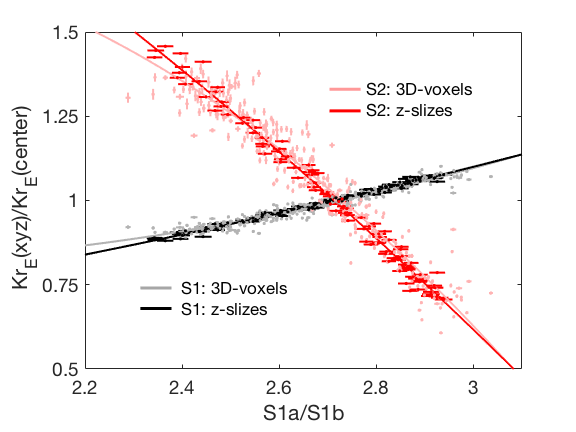
\includegraphics[scale=0.4]{figures/Fig5.png}
\captionof{figure}{The Z (black) and three dimensional (grey) relationship of the $^{83m}$Kr S1a/S1b ratio to the $^{83m}$Kr S1 field effect.  The black and grey data points are not measured, but instead inferred from the Z (dark red) and three dimensional (light right) relationship of the $^{83m}$Kr S1a/S1b ratio to the $^{83m}$Kr S2$_E$ field effect.}
 \label{fig:S1FieldFig}
\end{figure}

\subsection{Measuring the S1a/S1b Ratio to S1 Field Effect Relationship with the S1a Light Yield} \label{MatthewsIdea}

The relative light yield of the $^{83m}$Kr 32.1 keV decay, $^{83m}$Kr 9.4 keV decay, and $^{57}$Co 122 keV decay has been measured as a function of the light yield at an applied electric field divided by the light yield at zero electric field by Manalaysay, et al. in reference \cite{Manalaysay}.  We can combine NEST predictions for the light yield of the 122 keV $^{57}$Co line with the ratio of the light yield of the 32.1 keV $^{83m}$Kr line to the 122 keV $^{57}$Co line from reference \cite{Manalaysay} to convert the relative light yield measurements to absolute light yield measurements.  This results in an empirical formula for the absolute light yield of the $^{83m}$Kr 32.1 keV decay as a function of electric field given by
\begin{equation}
\frac{\gamma}{E} = 55.2[1-0.0004895 \times F \times \ln{(1 + 1/(8.9\mathrm{e}{-4} \times F))}]
\label{S1aYield}
\end{equation}
where $\gamma$ is the number of photons, $E$ is the energy of the decay, and $F$ is the applied electric field in units of V/cm.  

Using equation \ref{S1aYield} we can directly measure the strength of the field effect in the $^{83m}$Kr S1 data and relate it to the S1a/S1b ratio.  We begin by using the electric fields maps presented in reference~\cite{LuciesMaps} to estimate the electric field in the detector in September 2015.   The electric field map is converted to a map of the expected light yield at 32.1 keV using equation \ref{S1aYield}, assuming no detector inefficiency effects are present. The three dimensional spatial dependence of the light yield provides a direct measurement of the strength of the field effect in the S1a data, given by $\gamma(xyz)$/$\gamma(center)$.  Note that the strength of the field effect in the S1a data can help us derive the strength of the field effect in the combined S1 data, but the two are not equivalent.  Normalizing the field effect in the S1a data to the center of the detector, as shown in equation \ref{S1aNorm}, produces S1a$_F$ data which has spatial variation due to detector inefficiency effects only.  
\begin{equation}
S1a_F = S1a \frac{\gamma(center)}{\gamma(xyz)}
\label{S1aNorm}
\end{equation}
We measure the detector inefficiency effects in the S1a$_F$ data by dividing the detector into three dimensional voxels with X and Y width of 7 cm and Z width of 47 $\mu$Sec.  A Gaussian distribution is fit to the S1a$_F$ spectrum in each voxel, and the Gaussian mean is used to determine the spatial dependence of the S1a$_F$ data due to detector inefficiency effects alone.  Since the detector inefficiency effects are not dependent on the energy of an event, the spatial variation measured in the S1a$_F$ data is equivalent to the spatial variation in the combined S1 data due to detector inefficiency effects alone.  Therefore, we can use the spatial variation measured in the S1a$_F$ data to produce detector inefficiency corrected combined S1$_E$ data as shown in the equation
\begin{equation}
S1_E= S1 \frac{S1a_F(center)}{S1a_F(xyz)}.
\end{equation}
Any residual spatial variation in the detector inefficiency corrected combined S1$_E$ data is due to field effects in the combined $^{83m}$Kr S1 data alone.  We measure the strength of these field effects by again dividing the detector into three dimensional voxels with X and Y width of 7 cm and Z width of 47 $\mu$Sec.  A Gaussian distribution is fit to the S1$_E$ spectrum in each voxel, and the Gaussian mean is used to determine the spatial dependence of the S1a$_E$ data due to field effects alone.  At the same time, we use separate Gaussian distribution fits to the S1a and S1b data in each voxel to measure the spatial dependence of the S1a/S1b ratio.  Finally, we relate the S1a$_E$ Gaussian mean to the S1a/S1b ratio of each voxel and fit a second order polynomial which describes the strength of the field effect in the $^{83m}$Kr combined S1 signal to the data. (Figure \ref{S1aFieldEffect}) Note that the large systematic errors in the S1a/S1b ratio to field effect relationship is introduced by uncertainties in the field maps and systematic errors in the detector inefficiency corrections.  These errors a significantly reduced when extracting efficiency corrections from CH$_3$T data due to the lower energy, and therefore lower sensitivity to field effects.

\begin{minipage}{8.15cm}
\begin{center}
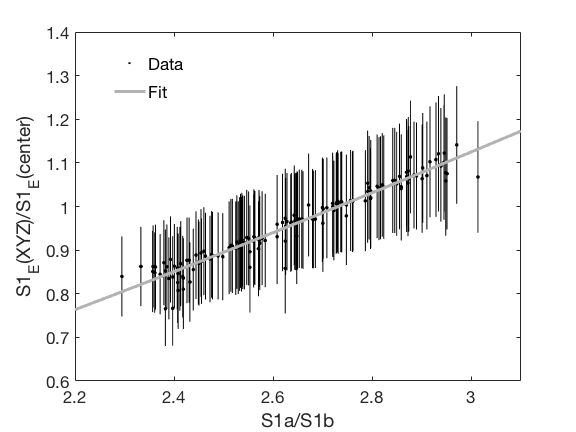
\includegraphics[scale=0.4]{figures/Fig6.png}
\captionof{figure}{The strength of the S1 field effect measured in this section (grey) compared to the strength of the S1 field effect measured in section \ref{section:S1relation2} (blue).  The large error bars on the data are due to systematic uncertainties in the field maps detector inefficiency corrections.}
\label{S1aFieldEffect}
\end{center}
\end{minipage}

\subsection{Measuring the S1a/S1b Ratio to S1 Field Effect Relationship with a $\chi^2$ Fitting Method} \label{section:S1relation2}

Although field induced variation in the recombination of a $^{83m}$Kr event can introduce a spatial and time dependence in the $^{83m}$Kr S1 and S2 signals, the total energy signal given (with gain factors $g_1$ and $g_2$) by 
\begin{equation} \label{CombinedEnergy}
E=\left(\frac{1}{73}\right)\left(\frac{S1_E}{g_1} + \frac{S2_E}{g_2}\right)
\end{equation}
should be insensitive to field variations.  We can take advantage of this fact to determine the optimal S1a/S1b to S1 field effect relationship corresponding to the directly measured S1a/S1b to S2 field effect relationship measured in section \ref{section:S1aS1b2}.  Unfortunately, we do not have knowledge of the strength of the field effect in the $^{83m}$Kr S1 signal, so we can not remove the field effect from the data to produce the efficiency-only corrected S1$_E$ signal.  Likewise, without efficiency corrected data we can not measure the gain factors $g_1$ and $g_2$ to produce a combined energy spectrum.  The only tools that we have at our disposal are a measurement of the strength of the field effect in the $^{83m}$Kr S2 signal and its relationship to S1a/S1b, as well as the ability to produce efficiency only corrected $^{83m}$Kr S2$_E$ data based on to the spatial variation of field effect corrected  $^{83m}$Kr S2$_F$ data.  In this section we turn to a $\chi^2$ minimization approach which will float the S1 field effect to S1a/S1b relationship, produce inefficiency corrections based on the field removed S1$_F$ and S2$_F$ signals, and then float the gain factors $g_1$ and $g_2$ to produce an optimized combined energy spectrum.  

We begin by eliminating one of the three parameters associated with the second order polynomial which describes the S1 field effect to S1a/S1b relationship.  We choose to normalize the spatial variation induced by the nonuniform electric field to the center of the detector, so the strength of the field effect as measured by $\frac{S1_{E,Kr}(xyz)}{S1_{E,Kr}(center)}$ must equal one at the center of the detector.  Therefore, we can relate one of the coefficients ($a$,$b$, and $c$) in the second order polynomial
\begin{equation}
 \frac{S1_{E,Kr}(xyz)}{S1_{E,Kr}(center)} = a\left(\frac{S1a}{S1b}\right)^2 + b\left(\frac{S1a}{S1b} \right) + c
 \end{equation}
 to the other two, such that
 \begin{equation}
 c=1-a\left(\frac{S1a_c}{S1b_c}\right)^2-b\left(\frac{S1a_c}{S1b_c}\right)
 \end{equation}
 where $S1a_c$ and $S1b_c$ represent the values of $S1a$ and $S1b$ at the center of the detector.  Next, we scan over a range of $a$ and $b$ values and produce the $\frac{S1_{E,Kr}(xyz)}{S1_{E,Kr}(center)}$ to $\frac{S1a}{S1b}$ relationship for each pair of $a$ and $b$ values.  We follow the procedure described in section \ref{KrypCalCode} and use the S1 field effect to S1a/S1b relationship from each pair of $a$ and $b$ values, in conjunction with the S2 field effect S1a/S1b relationship measured in \ref{section:FieldEffects}, to produce efficiency-only corrections for CH$_3$T data and $^{83m}$Kr data from September 2015 and February 2016. These corrections are used to produce S2$_E$ and S1$_E$ data for all four data sets.  We then scan over a range of $g_1$ and extraction efficiency (EE) values and use the S2$_E$ and S1$_E$ data to produce a combined energy spectrum (for each source) for each combination of $a$,$b$,$g_1$, and EE based on equation \ref{CombinedEnergy}.  Note that $g_2=SE \times EE$, where $SE$ is the single electron size at the time of each data set.  

To evaluate the performance of each $a$,$b$,$g_1$, and $EE$ combination we must develop models for the expected energy spectra of CH$_3$T and $^{83m}$Kr data in September 2015 and February 2016.  The $^{83m}$Kr events consist of a mono-energetic 32.1 keV decay and a mono-energetic 9.4 keV decay.  The expected energy spectrum is a Gaussian distribution centered around the sum of these two mono-energetic decays at 41.55 keV.  The width of the Gaussian distribution depends on a number of factors, including the detector's efficiency for collecting S1 and S2 light, as well as the spatial dependence of the recombination of $^{83m}$Kr events induced by the nonuniform electric field.  While we can measure most of these parameters, we would have to feed them into NEST to determine the final width of the Gaussian distribution.  Since NEST does not simulate $^{83m}$Kr events well, we can only use the mean of the Gaussian distribution as a figure of merit for the $^{83m}$Kr energy spectrum.

Tritium is a beta decay with an energy spectrum that has a broad peak at 2.5 keV and a smoothly falling distribution out to 18 keV.  As with $^{83m}$Kr, this spectrum is smeared based on a number of parameters.  Unlike $^{83m}$Kr, the smearing in CH$_3$T data can be accurately determined by NEST so we can compare the energy spectrum from data to simulations on a bin by bin basis. 

For each $a$,$b$,$g_1$, and $EE$ combination a reduced $\chi^2$ for the CH$_3$T and $^{83m}$Kr data is measured using the difference between the expected energy spectra and measured energy spectra.   During the $^{83m}$Kr $\chi^2$ calculation, the energy spectrum is from each point in time is divided into drift time bins so that the spatial dependence of the energy spectrum is included in the $\chi^2$ measurement.  The $^{83m}$Kr data has very high statistics, and only the mean of a Gaussian fit to the data is of interest, so the variance used in the $\chi^2$  measurement  is dominated by systematic error.  We use the standard deviation of the $^{83m}$Kr energy spectrum over the duration of Run03 to evaluate the size of this systematic error, and find $\sigma = 0.2395$.  During the CH$_3$T $\chi^2$  calculation, the energy spectrum is divided into energy bins so that the entire beta spectrum (above 3.5 keV to avoid the detector threshold) is included in the $\chi^2$ measurement.  The variance of the CH$_3$T data is based on statistics alone, due to finer binning and lower statistics of the data.  We choose to define a total reduced $\chi^2$ (to be minimized in the $\chi^2$ fit) as the average of the reduced $\chi^2$ for the $^{83m}$Kr and CH$_3$T data, so that each source carries the same amount of weight in the fit. A minimum average reduced  $\chi^2$ of 0.8413 is found for the best fit parameters of $a=0.065 \pm 0.0117$,$b=0.020 \pm 0.060$,$g_1=0.0980 \pm 0.001$, and $EE=0.808 \pm 0.029$. The corresponding value of the zeroth order coefficient is $c=0.461 \pm 0.186$.  The reduced $\chi^2$ of the $^{83m}$Kr and CH$_3$T energy spectra separately are 12.17/26=0.4682 (p=0.99) and 150.6/124=1.2143 (p=0.05), respectively. Note that (as we will see in section \ref{Results}) the extraction efficiency needed to produce these results is consistent with our expectations, and the results produce $^{83m}$Kr energy peaks (unbinned in drift time) that are within one sigma of the expected 41.55 keV in both September 2015 and February 2016. 


\subsection{Summary of S1a/S1b Ratio to Field Effect Measurements}

We have directly measured the strength of the field effect in $^{83m}$Kr S2 data by removing detector inefficiency effects from the data with the help of CH$_3$T data.  We have also used a $\chi^2$ optimization methods to find the optimal S1 field effect to S1a/S1b relationship to pair with the direct S2 field effect measurement.  We find that the optimal S1 field effect found by a $\chi^2$ optimization agrees very closely with our expectations from recombination physics, and from the expected light yield of the $^{83m}$Kr S1 data 32.1 keV decay.   We choose to use the S2 field relationship measured in section \ref{section:S1aS1b2} and the corresponding optimal S1 field effect relationship measured in section \ref{section:S1relation2} for our work.  The polynomials that describe these relationships are:
\begin{multline}
\frac{S2_{E,Kr}(xyz)}{S2_{E,Kr}(center)} =   \\ -0.499 \left(\frac{S1a}{S1b} \right)^2 + 1.48  \left(\frac{S1a}{S1b} \right) + 0.667
\end{multline}
\begin{multline}
\frac{S1_{E,Kr}(xyz)}{S1_{E,Kr}(center)} = \\  0.065 \left(\frac{S1a}{S1b} \right)^2 + 0.020 \left(\frac{S1a}{S1b} \right) + 0.461
\end{multline}


\begin{center}
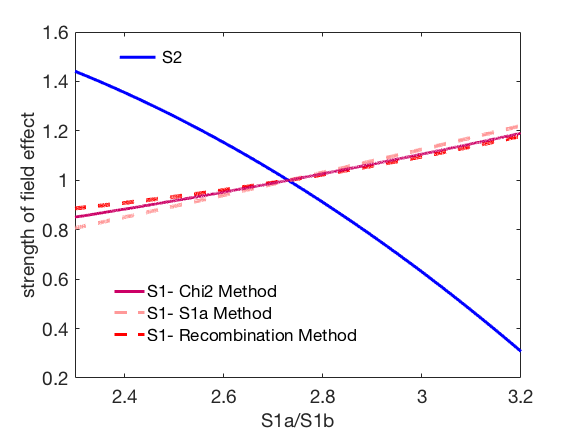
\includegraphics[scale=0.4]{figures/Fig7.png}
\captionof{figure}{The S1a/S1b to field effect relationships measured in this work.  The method to measure each line is indicated by the color in the legend.  Red shades indicate measurements of the strength of the field effect in  $^{83m}$Kr S1 data, and blue shades indicate the strength of the field effect in  $^{83m}$Kr S2 data. Solid lines represent measurements that are used in KrypCal, and dashed lines represent measurements that are supplementary cross checks. }
 \label{AllMeasurements}
\end{center}


